\documentclass[journal=jpccck,manuscript=article]{achemso}

\usepackage{hyperref}

\usepackage{siunitx}
\DeclareSIUnit\rydberg{Ry}
\usepackage{tikz}
\usepackage{paralist}
\usepackage[version=4]{mhchem}
\usepackage{booktabs}
\usepackage{rotating}
\usepackage{chngcntr}


\author{Pierre Beaujean}
\affiliation[Unamur]
{University of Namur, Theoretical Chemistry Lab, Unit of Theoretical and Structural Physical Chemistry, Namur Institute of Structured Matter, rue de Bruxelles, 61, B-5000 Namur (Belgium)}


\author{Benoît Champagne}
\affiliation[Unamur]
{University of Namur, Theoretical Chemistry Lab, Unit of Theoretical and Structural Physical Chemistry, Namur Institute of Structured Matter, rue de Bruxelles, 61, B-5000 Namur (Belgium)}
\email{benoit.champagne@unamur.be}

\title{Prediction of XPS binding energies for molecules grafted on calcium surfaces}

\def\dbe{\ensuremath{\Delta\text{BE}}}

\begin{document}
\maketitle

\section{Introduction}

Batteries represent a crucial technology for the transition to a climate-neutral society. Since their market introduction, lithium-ion batteries (LIBs) have evolved into a highly mature technology, currently utilized in a wide range of applications. Despite their established performance, LIBs face significant limitations that hinder their suitability for large-scale applications, primarily due to three fundamental issues:
\begin{inparaenum}[(i)] 
	\item limited availability of raw materials, 
	\item insufficient energy density, and 
	\item inadequate sustainability across an extended number of cycles. 
\end{inparaenum}

Addressing the second point can be achieved through the use of divalent cations, such as \ce{Ca^2+}. However, its elevated reactivity demands the design of specialized electrolytes to support a reversible mechanism. Additionally, detailed insight into the chemistry of the solid-electrolyte interphase (SEI) remains crucial.
In the literature, calcium-ion batteries (CIBs) utilize electrolytes such as dimethyl ether (DME), ethylene carbonate (EC), glyme, or tetrahydrofuran (THF), often in combination with weakly coordinating anions like \ce{BH4-} or \ce{BF4-} \cite{zhaoRevealingSolidElectrolyte2022,taghavi-kahaghPoweringFutureComprehensive2023}. Although both experimental \cite{melemedImpactDifferentialCa22023} and quantum chemistry \cite{hahnCriticalRoleConfigurational2020,liepinyaComputationalComparisonEther2021,pathreekerWhyTetrahydrofuranGood2021,yamijalaStabilityCalciumIon2021} studies on SEI formation exist, greater insight can be gained by combining experimental spectra with theoretical calculations.


X-ray photoelectron spectroscopy (XPS) is a surface-sensitive, quantitative spectroscopy that allows for the identification of elements within the material or at its surface. It belongs to the family of photoemission spectroscopies, where the energy of electrons emitted by the photoelectric effect is analyzed. Specifically, XPS uses a beam of soft X-rays ($\SI{100}{\electronvolt} < h\nu < \SI{10}{\kilo\electronvolt}$), enabling the probing of core electrons (low principal quantum number) \cite{stevieIntroductionXrayPhotoelectron2020}. It is routinely used to gain understanding on the SEI composition, both experimentally \cite{melemedImpactDifferentialCa22023} and with calculations \cite{ebadiInsightsLiMetalOrganic2019}.

This study investigates the XPS spectra associated with the degradation and polymerization of THF, using it as a model system. Various potential degradation products (Fig.~\ref{fig:THFdegradation}), as well as the polymerization into poly(tetramethylene ether) glycol (PTMEG), are examined on different calcium substrates, including calcium oxide and calcium hydride.


\begin{figure}
	\centering
	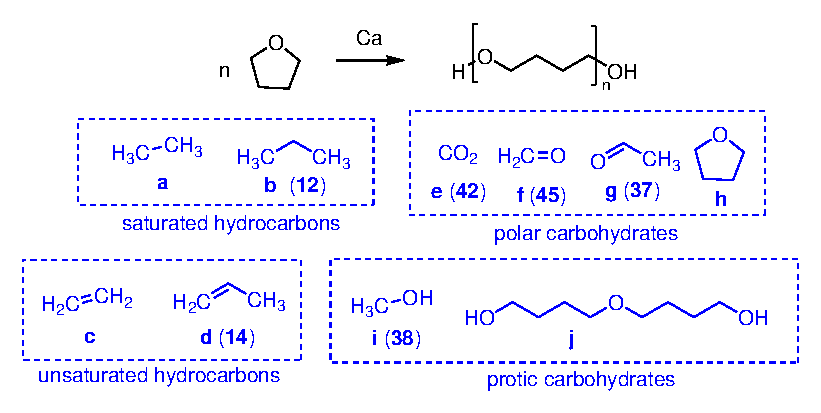
\includegraphics{Figure1}
	\caption{The main polymerization pathway of THF leads to PTMEG (black). \textbf{j} is used as a model for the PTMEG, while fragmentation can lead to (un)saturated hydrocarbons (\textbf{a}-\textbf{d}) or carbohydrates (\textbf{e}-\textbf{i}).}
	\label{fig:THFdegradation}
\end{figure}

\section{Theoretical methods}

In XPS spectroscopy, the conservation of energy is described by the equation:
\begin{equation}
	h\nu = \text{BE} + E_{\text{kin}} + \phi, \label{eq:xps}
\end{equation}
where BE is the binding energy of the electron, $E_{\text{kin}}$ is the kinetic energy of the emitted electron (measured by the detector), and $\phi$ is the work function, which accounts for surface effects and detector contributions. Using a source of monochromatic X-rays (such as Al $K_\alpha$, $h\nu = \SI{1486.7}{\electronvolt}$), it is possible to determine BE from $E_{\text{kin}}$ \cite{vinesPredictionCoreLevel2018}. The binding energy depends on how tightly the electron is bound in its orbital, making it sensitive to the oxidation state and chemical environment of the originating atom. Generally, more electronegative surroundings result in higher BE, providing information on the atom's environment, much like chemical shifts in NMR.

From a quantum chemistry perspective, binding energy is akin to the ionization energy of core electrons:
\begin{equation}
	\text{BE}_i = E^{N-1}_i(\text{final}) - E^{N}(\text{initial}), \label{eq:dscf}
\end{equation}
where $E^{N}$ and $E^{N-1}_i$ are the energies of the initial $N$-electron non-ionized state and the final $N-1$ electron ionized state with a core hole on atom $i$. While these energies could be obtained through (relativistic) multi-configuration approaches, this is impractical for large systems. Even CIS or TD-DFT based calculations of excitation energies are challenging, as they correspond to highly excited states \cite{vinesPredictionCoreLevel2018}.

For gas-phase molecules, classical quantum chemistry tools can be utilized. At the HF level, core-level BE can be approximated using Koopmans' theorem, which correlates BEs to the orbital energy of the removed electron. This is known as the initial state (IS) or frozen orbitals (FO) approach. However, electronic relaxation effects are neglected. More accurate values can be obtained using Eq.~\eqref{eq:dscf}, by computing the energy difference between initial and final states at the HF level, known as the $\Delta$SCF approach, which includes final state (FS) effects. While this method may provide quantitative agreement in some cases, electron correlation effects are significant, necessitating the use of density functional theory (DFT), for which Koopmans' theorem no longer applies \cite{pueyobellafontPredictionCoreLevel2015,pueyobellafontPredictingCoreLevel2017}.

Treating solids or surfaces adds further complexity. Generally, only valence levels are explicitly treated, with pseudopotentials (PPs) modeling core electrons. The projected augmented wave (PAW) method maps results to all-electron wavefunctions using specially designed PPs and transformations \cite{blochlProjectorAugmentedwaveMethod1994}. A core hole can be generated, neglecting the relaxation of other core electrons but including valence electron relaxation. This limits the accuracy of absolute BE descriptions.
A complementary challenge arises due to the use of periodic boundary conditions (PBC), since the core hole is periodically repeated, creating an infinitely charged system. Two approaches can address this: 
\begin{inparaenum}[(i)]
	\item add the excited electron to the bottom of the conduction band (or LUMO for isolated molecules), or 
	\item remove the excited electron from the system and use a background counter-charge.
\end{inparaenum}
The first approach underestimates BEs, resembling absorption processes, while the second induces physically incorrect effects, further complicating absolute BE prediction.\cite{olovssonCorelevelShiftsComplex2006}

However, relative BE can be estimated by computing wavefunctions for a fractional number of electrons using Slater transition state theory and Janak's theorem \cite{janakProofThatFrac1978}, resulting in the Slater-Janak (SJ) approach \cite{hiraoImprovedSlaterTransition2021}. In this work, BE are computed with a half-electron placed either in the conduction band or in the vacuum, referred to as the SJ and SJ\textsuperscript{n} approaches\cite{pueyobellafontPredictingCoreLevel2017}, respectively (Fig.~\ref{fig:method}).
	
	\begin{figure}[!h]
		\centering
		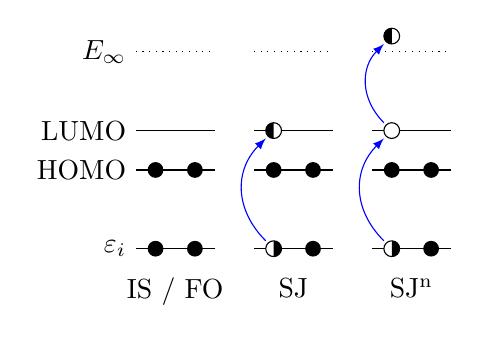
\begin{tikzpicture}
			\draw (0,0) node[left]{$\varepsilon_i$}-- node[midway,below=.25cm]{IS / FO} +(1,0);
			\draw (0,1) node[left]{HOMO}-- +(1,0);
			\draw (0,1.5) node[left]{LUMO}-- +(1,0);
			\draw[dotted] (0,2.5) node[left]{$E_\infty$}-- +(1,0);
			\fill (.25,0) circle (.1cm);
			\fill (.75,0) circle (.1cm);
			\fill (.25,1) circle (.1cm);
			\fill (.75,1) circle (.1cm);
			
			\begin{scope}[xshift=1.5cm]
				\draw (0,0) -- node[midway,below=.25cm]{SJ} +(1,0);
				\draw (0,1) -- +(1,0);
				\draw (0,1.5) -- +(1,0);
				\draw[dotted] (0,2.5) -- +(1,0);
				\draw[fill=white] (.25,0) circle (.1cm);
				\fill (.25,-.1) arc (-90:90:.1);
				\fill (.75,0) circle (.1cm);
				\fill (.25,1) circle (.1cm);
				\fill (.75,1) circle (.1cm);
				\draw[fill=white] (.25,1.5) circle (.1cm);
				\fill (.25,1.4) arc (-90:-270:.1);
				\draw[-latex,blue] (.15,.1) .. controls +(-.4,.4) and +(-.4,-.4) .. (.15,1.4);
			\end{scope}
			
			\begin{scope}[xshift=3cm]
				\draw (0,0) -- node[midway,below=.25cm]{SJ\textsuperscript{n}} +(1,0);
				\draw (0,1) -- +(1,0);
				\draw (0,1.5) -- +(1,0);
				\draw[dotted] (0,2.5) -- +(1,0);
				\draw[fill=white] (.25,0) circle (.1cm);
				\fill (.25,-.1) arc (-90:90:.1);
				\fill (.75,0) circle (.1cm);
				\fill (.25,1) circle (.1cm);
				\fill (.75,1) circle (.1cm);
				\draw[fill=white] (.25,1.5) circle (.1cm);
				\draw[-latex,blue] (.15,.1) .. controls +(-.4,.4) and +(-.4,-.4) .. (.15,1.4);
				\draw[-latex,blue] (.15,1.6) .. controls +(-.3,.3) and +(-.3,-.3) .. (.15,2.6);
				\draw[fill=white] (.25,2.7) circle (.1cm);
				\fill (.25,2.6) arc (-90:-270:.1);
			\end{scope}
		\end{tikzpicture}
		\caption{Approaches to compute BE as the energy of the molecular orbital where the core hole is located: initial state (IS, also referred to as frozen orbitals, FO) and Slater-Janak (SJ). When the electron is further removed from the system (and conceptually pushed to the vacuum, $E_\infty$), JS\textsuperscript{n} is noted. Adapted from Ref.~\citenum{pueyobellafontPredictingCoreLevel2017}.}
		\label{fig:method}
	\end{figure}

Finally, while the determination of absolute binding energies (BE) is challenging from a theoretical perspective, the measurement or calculation of the work function, $\phi$ in Eq.~\eqref{eq:xps}, is also complex. As a result, both experimentalists and quantum chemists often focus on the relative binding energy, $\Delta\text{BE}$, which is the difference in binding energy for a given atom with respect to a reference compound \cite{vinesPredictionCoreLevel2018}. In this contribution, relative BE values are computed as:\begin{equation}
	\Delta\text{BE}_i = \text{BE}_i - \text{BE}(\text{ref}), \label{eq:dbe}
\end{equation} 
using the calculated or experimental BE values for \ce{CH4}, \ce{NH3}, \ce{H2O}, \ce{B2H6}, and \ce{HF} as references for carbon, nitrogen, oxygen, boron, and fluorine, respectively. The experimental values are taken from Ref.~\citenum{pueyobellafontPredictingCoreLevel2017}. For calcium, the innermost atom of a 1x1 Ca slab containing 16 layers (\textit{vide infra}) is used as reference.

	
\section{Computational details}

Unless otherwise stated, all calculations were performed using the PBE-D3 level of theory with VASP (version 6.4.1) and the projector-augmented wave (PAW) method \cite{blochlProjectorAugmentedwaveMethod1994}. The energy convergence criterion was set to \SI{e-4}{\electronvolt}, with a cutoff of \SI{550}{\electronvolt} for the kinetic energy of the plane waves. Gaussian smearing of the energy of valence electrons, with a width of \SI{0.2}{\electronvolt}, was applied. Brillouin zone integration was performed at the $\Gamma$-point for molecules in the gas phase, using a 4x4x4 Monkhorst-Pack k-point mesh\cite{monkhorstSpecialPointsBrillouinzone1976} for bulk calculations, and a 4x4x1 mesh for slab calculations. The \texttt{Ca\_sv} pseudopotential\cite{blochlProjectorAugmentedwaveMethod1994,kresseUltrasoftPseudopotentialsProjector1999} was employed to model calcium.

All optimizations were carried out using the Limited-memory Broyden-Fletcher-Goldfarb-Shanno  (L-BFGS) algorithm, driven by the Atomic Simulation Environment (ASE) package \cite{larsenAtomicSimulationEnvironment2017}, using VASP energies and forces as inputs, until the force on all atoms was below \SI{e-2}{\electronvolt\per\angstrom}.

For the calculation of binding energies (BE), VASP allows targeting a specific orbital, $i$, by removing half an electron from it. For SJ calculation, dipole corrections (using the \texttt{IDIPOL} keyword) are included. For SJ\textsuperscript{n} calculations, it is necessary to adjust the total number of valence electrons (by default, half an electron is added; see Fig.~\ref{fig:method}) using the \texttt{NELECT} keyword. After the calculation, the corresponding eigenvalue, $\varepsilon_i\left(\frac{1}{2}\right)$, is extracted. The binding energy is then calculated as:
\begin{equation}
	\text{BE}_i = 
	E_{ref}- \varepsilon_i\left(\tfrac{1}{2}\right), \label{eq:xpsbe}
\end{equation}
where $E_{ref}$ is a reference energy, chosen to ensure consistency across systems. This study considers several choices for $E_{ref}$:
\begin{enumerate}
	\item $E_{ref}=0$, thus using only the orbital energy,
	\item $E_{ref}=E_F$, where the Fermi energy $E_F$ is used, computed with \texttt{EFERMI = MIDGAP} in the VASP input to account for Gaussian smearing,
	\item $E_{ref}=E_\infty$, the vacuum energy, calculated by taking the electrostatic potential in the vacuum region of the cell (when dipole correction are included, the vacuum potential is not equal in both side of the slab, the average value is considered),
	\item $E_{ref}=\phi$, where the work function $\phi = E_\infty - E_F$ is considered\cite{kahnFermiLevelWork2015}, and
	\item $E_{ref}= \varepsilon_{ref}$, where $\varepsilon_{ref}$ is the orbital energy of another atom in the cell. Although it might seem reasonable to use calcium, which is present in all slabs, this approach would depend on the slab's nature and would be not possible for gas-phase molecules. To overcome this, an Argon atom (to mimic calcium) is placed in the vacuum region, and $\varepsilon_{ref}=\varepsilon_{Ar,2s}$.
\end{enumerate}
It should be noted, however, that extracting $E_\infty$ is not feasible for bulk systems, where no vacuum region exists, or for charged systems, where the electrostatic potential is not constant in the vacuum region. This latter condition occurs when employing the SJ\textsuperscript{n} method. It is however possible to correct the Fermi level energy to remove the impact of the background of charge, as discussed in Ref.~\citenum{lozovoiInitioSimulationCharged2001}. This possibility is referred to as $E_{ref}=E_F'$, where $E_F' = E_F - \max\{E_{elst}(z)\}$, with $E_{elst}(z)$ being the planar average of the electrostatic potential along the $z$ axis.


To obtain a spectrum, a Gaussian function centered at each computed \dbe{} is used. Unless otherwise specified, a root mean square width, $\sigma = \SI{0.2}{\electronvolt}$ is employed.

\paragraph{Binding energies of molecules in the gas phase.}
To assess the accuracy of the SJ and SJ\textsuperscript{n} methods and the choice of $E_{ref}$, the results from Belafont \textit{et al.} \cite{pueyobellafontPredictingCoreLevel2017}, which compare experimental and theoretical calculations (computed at the same level of approximation as ours) of gas-phase \dbe, are replicated. Their dataset comprises 184 experimental absolute binding energies (BEs) from 68 molecules, including carbon (N=107), nitrogen (N=20), oxygen (N=22), boron (N=20), and fluorine (N=15) atoms (Fig.~\ref{fig:core185}). Following a geometry optimization, each molecule is placed in a cubic box with a side length of \SI{20}{\angstrom}, and the \dbe{} are computed for each atom of interest.


\begin{figure}[!h]
	\centering
	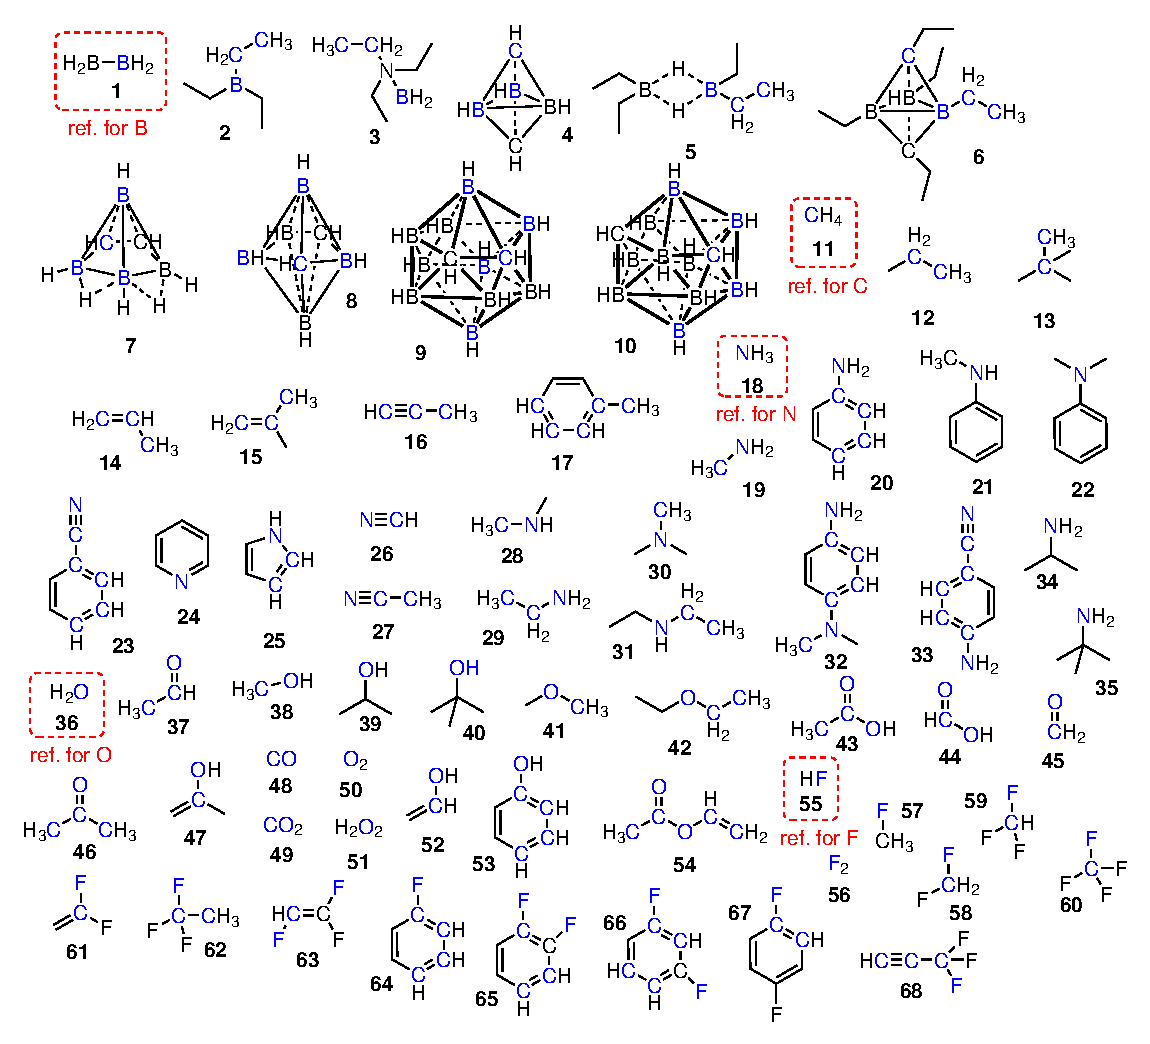
\includegraphics[width=\linewidth]{Figure3}
	\caption{Molecules for the benchmark \cite{pueyobellafontPredictingCoreLevel2017}. The atoms for which experimental BE are provided are highlighted in blue.  The reference compounds used for each atom are highlighted in red.}
	\label{fig:core185}
\end{figure}

\paragraph{Binding energies of molecules grafted on surfaces.} The binding energies (\dbe{}) of molecules adsorbed on surfaces are investigated following the protocol established by Ebadi and co-workers \cite{ebadiInsightsLiMetalOrganic2019}. Initially, bulk Ca (from the Material Project, \texttt{MP-45}), CaO (\texttt{MP-2605}), and \ce{CaH2} (\texttt{MP-23713}) were selected, and their atomic positions and cell parameters were optimized.

Subsequently, to determine the optimal surface orientation, 1x1 slabs with increasing thickness along different low-index orientations [(100), (110), and (111)] were constructed using ASE \cite{larsenAtomicSimulationEnvironment2017}. The slabs were relaxed with the central two layers frozen to mimic bulk conditions, with the distance between slab repetitions set to 10 times the $c$ cell parameter of the bulk. For each orientation, the surface energy $\gamma^{hkl}$ was calculated by least-squares fitting of the following expression \cite{sunEfficientCreationConvergence2013,tranSurfaceEnergiesElemental2016}:
\begin{equation}
	E^{hkl}(N) = E_0\,N + 2A\,\gamma^{hkl} \label{eq:surf}
\end{equation}
where $N$ is the number of layers in the slab, $A$ is the slab surface area, $E^{hkl}(N)$ is the energy of the relaxed slab cut along $(hkl)$, and $E_0$ approximates the energy of one layer. The results (Table \ref{tab:surf}, Fig.~\ref{fig:surf}) indicate that (100) surfaces are the most energetically favorable, consistent with the literature \cite{deleeuwDensityFunctionalTheory2000,ebadiInsightsLiMetalOrganic2019}.

\begin{table}[!h]
	\centering
	\begin{tabular}{lccc}
		\toprule
		&	\ce{Ca} & \ce{CaO} &	\ce{CaH2} \\
		\midrule
		(100) & 0.555 ($N\in[6,16]$) & 0.470 ($N\in[6,16]$) & 0.871  ($N\in[12,32]$)\\
		(110) & 0.630  ($N\in[6,16]$)& 1.777  ($N\in[6,16]$)& 1.109 ($N\in[12,32]$)\\
		(111) & 0.563  ($N\in[6,16]$) & 4.080  ($N\in[5,15]$)  & 1.117   ($N\in[12,32]$) \\ 
		\bottomrule
	\end{tabular}
	\caption{Surface energies ($\gamma^{hkl}$, in \si{\joule\per\meter\squared}) of Ca, CaO, and \ce{CaH2} slabs along different orientations, as determined through Eq.~\eqref{eq:surf} using the $N$ values given in parentheses.}
	\label{tab:surf}
\end{table}

Using the (100) orientation, 3x3 slabs (consisting of 6 layers, with a vacuum of \SI{20}{\angstrom} between two slab repetitions) were created and relaxed (with frozen cell parameters). Additionally, given that it reported to be favorable\cite{deleeuwDensityFunctionalTheory2000,fujimoriInteractionWaterCaO2016a}, the adsorption of water on the CaO surface was investigated: an additional slab with full coverage (1 water molecule per surface Ca), denoted as \ce{CaO.H_2O}, was built and its geometry was optimized. 

Finally, compounds \textbf{a}-\textbf{j} (Fig.~\ref{fig:THFdegradation}) were introduced on both sides of the slab (initially approximately \SI{6}{\angstrom} away from the surface), followed by a final optimization (with frozen cell parameters, and the two central layers kept frozen). Subsequently, binding energies were computed for each relevant atom.

\section{Results}

\subsection{Biding energies in gas phase}

A comparison between experimental and computed \dbe\ is presented in Fig.~\ref{fig:xps_C185}. The agreement with previous investigations \cite{pueyobellafontPredictingCoreLevel2017,golzeAccurateAbsoluteRelative2020} shows that the SJ\textsuperscript{n} protocol provides reliable results for all atoms, with very small mean errors (<\SI{0.1}{\electronvolt}) and acceptable standard deviations (0.1 to \SI{0.4}{\electronvolt}). However, it should be noted that a reference per atom is necessary (Table \ref{tab:xpssjn}), as the difference between experimental and computed absolute BE increases with the atomic number. 
In contrast, the SJ protocol exhibits non-systematic errors, as indicated by the large standard deviations (>\SI{0.7}{\electronvolt}).


\begin{figure}[!h]
	\centering
	 \includegraphics[width=.8\linewidth]{Figure4}
	 \caption{Comparision between experimental and calculated gas phase \dbe{}, as computed with the SJ (blue) and SJ\textsuperscript{n} (orange) protocols on the different atoms. For each of them, the error (as mean $\pm$ standard deviation) for both protocols is given.}
	 \label{fig:xps_C185}
\end{figure}

\begin{table}[!h]
	\centering
	\begin{tabular}{lcccc}
		\toprule
		& Reference & BE (exp.)  & BE (SJ\textsuperscript{n})  & $\Delta$(SJ\textsuperscript{n}- exp.)\\
		\midrule
		B 1s & \ce{(BH2)2} & 196.50 & 201.47 & 4.97\\
		C 1s & \ce{CH4} & 290.90 & 297.04 & 6.14\\
		N 1s & \ce{NH3} & 405.60 & 413.58 & 7.98\\
		O 1s & \ce{H2O} & 539.70 & 548.79 & 9.09\\
		F 1s & \ce{HF} & 694.23 & 704.78 &10.55\\
		\bottomrule
	\end{tabular}
	\caption{Comparison between experimental (from Ref.~\citenum{pueyobellafontPredictingCoreLevel2017}) and calculated (as computed with the SJ\textsuperscript{n} protocol) absolute BE.}
	\label{tab:xpssjn}
\end{table}

\clearpage
These results also indicate that the \dbe{} can serve as a measure of the local chemical environment. As shown in Fig.~\ref{fig:trends}, three key factors can impact \dbe{}: \begin{inparaenum}[i)]
	\item the hybridization of the atom, which plays a moderate role in this set of compounds,
	\item the electronegativity of neighboring atoms, which generally increases the binding energy or carbon (as observed with carbon), and
	\item the number of electronegative neighbors, as demonstrated, for example, in the \ce{CF_xH_{4-x}} series (\textbf{11}, \textbf{57}-\textbf{60}), where \dbe{} increases by \SI{10}{\electronvolt} from $x=0$ (\ce{CH4}) to $x=4$ (\ce{CF4}).
\end{inparaenum}
The second and third effects combine to produce large binding energies (in comparison to the reference) in compounds containing oxygen and fluorine. On the other hand, the binding energies for boron are systematically smaller than the reference, \textbf{1} (\ce{B2H4}), thought carbon has a larger electronegativity than boron.



\begin{figure}[!h]
	\centering
	\includegraphics[width=\linewidth]{Figure5}
	\caption{ Trends among \dbe{} for of \textbf{1}-\textbf{67} (as computed with the SJ\textsuperscript{n} protocol). Each bar represent the minimum and maximum \dbe{} computed for each atom, with a given hybdrization (C, N, O) and neighbors (C).}
	\label{fig:trends}
\end{figure}

\clearpage
\subsection{Binding energies of bare slabs}

Although the SJ\textsuperscript{n} protocol performs better in the gas phase, literature recommends using the SJ protocol for solids, as it correctly reproduces experimental trends \cite{olovssonCorelevelShiftsComplex2006}. An alternative approach, the final state (FS) scheme, can also be used, where one electron is added to the valence band instead of $\frac{1}{2}$ as in the SJ protocol \cite{trinhEvaluatingStructureCatalysts2013a,vandenbosscheEffectsNonlocalExchange2014}.

The impact of slab thickness on the resulting spectra is therefore assessed using the SJ protocol, as shown in Fig.~\ref{fig:slabsthickness}. Increasing slab thickness shifts the balance between surface and bulk features towards the latter, but it does not significantly change the peak positions. Therefore, further calculations can safely use slabs with the fewest number of layers to save computation time.


\begin{figure}[!h]
	\centering
	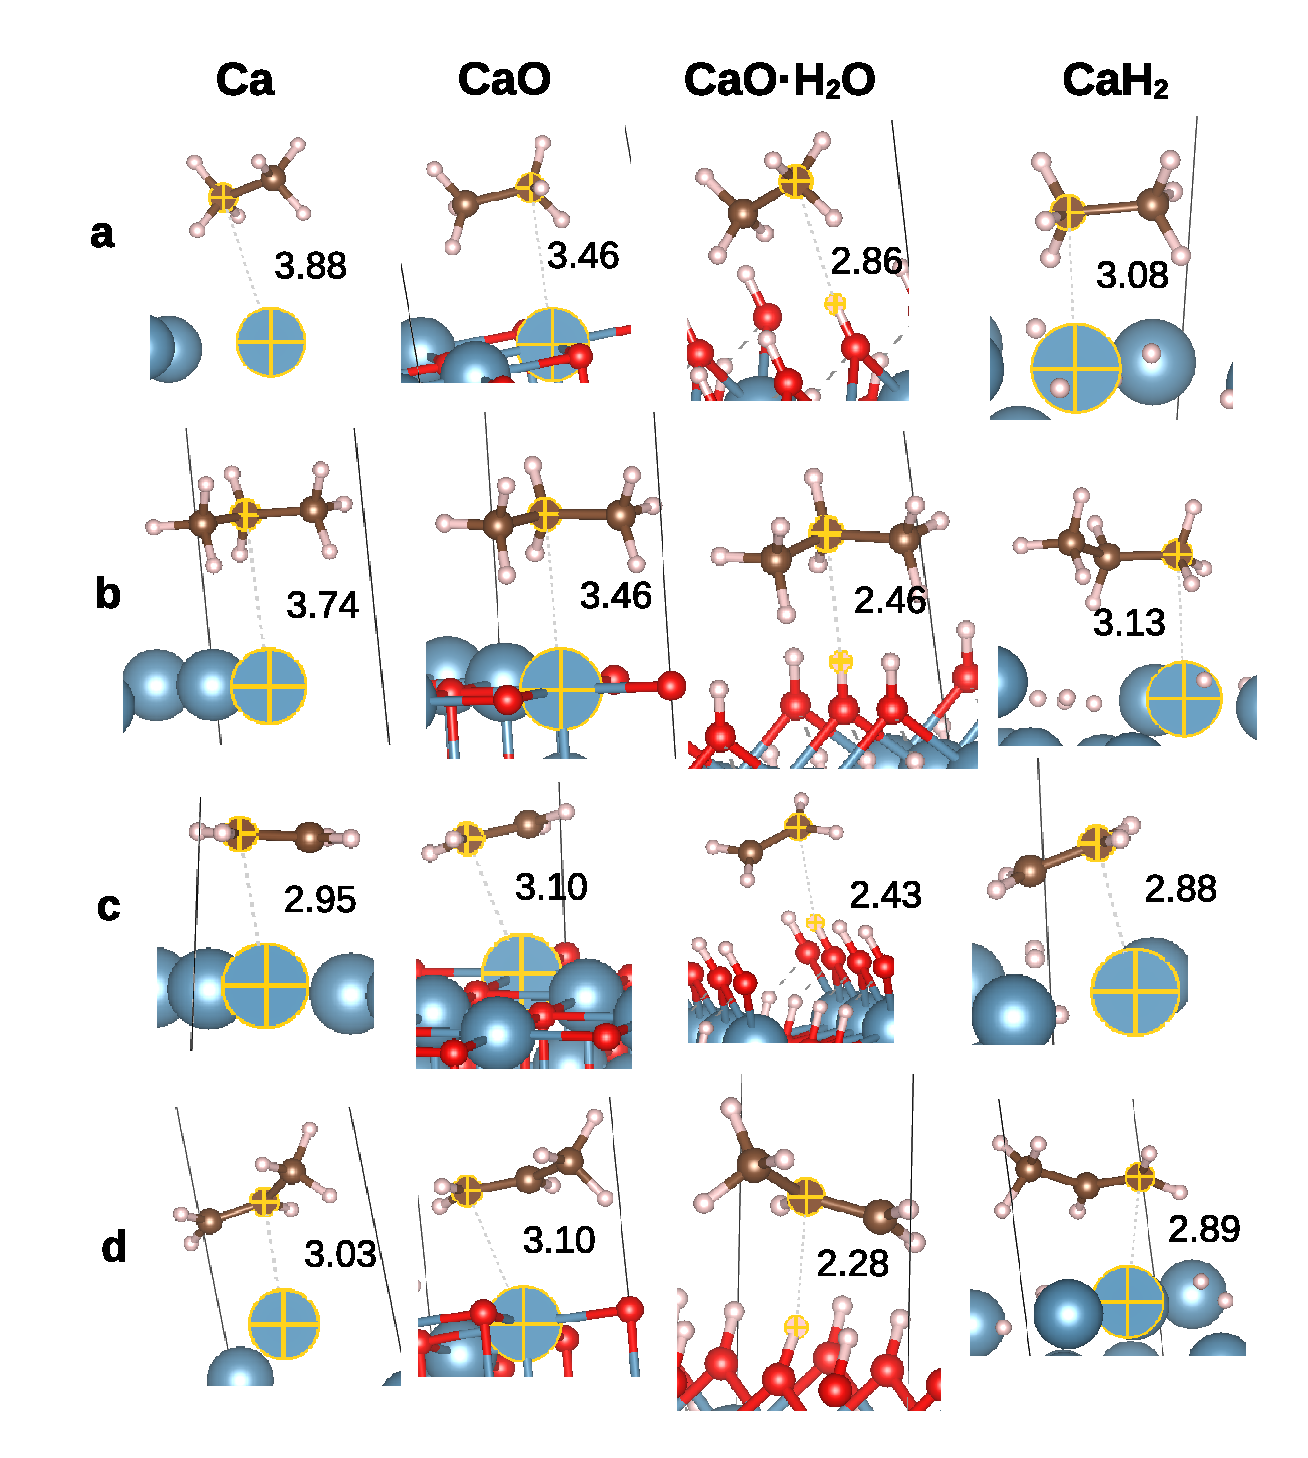
\includegraphics[width=\linewidth]{Figure6}
	\caption{Impact of the slab thickness (indicated as the number of layers) on the resulting XPS spectra (as computed with the SJ protocol).}
	\label{fig:slabsthickness}
\end{figure}

A comparison with the SJ\textsuperscript{n} protocol (Fig.~\ref{fig:slabsthicknessSJn}) shows that while the Ca 2s binding energies are similar with both protocols, differences in the shape of the spectra appear for Ca 2s in \ce{CaH2} (where bulk and surface features are more pronounced) and for O 1s in CaO (where the difference between bulk and surface is less significant). Notably, the SJ\textsuperscript{n} protocol predicts a difference of \SI{7.6}{\electronvolt} between the reference (water, for O 1s) and the value of O 1s in \ce{CaO}, which is close to the experimental value of \SI{7.8}{\electronvolt} \cite{cristHandbookMonochromaticXPS1999}. In contrast, the SJ protocol predicts a difference of only \SI{5}{\electronvolt}.\footnote{Cette comparaison est dangereuse, voire casse-gueule. En effet, le résultat en phase gas n'as pas été \textit{shifté} par $E_F$, le résultat pour le slab, oui. Donc....?}

\subsection{Adsorption on slab: geometrical and energetic aspects}

The optimized geometries of compounds \textbf{a}-\textbf{j} adsorbed on slabs are shown in Figs.~\ref{fig:distsad}-\ref{fig:distsij}. The interaction energy, calculated as $\Delta E_{int} = E_{X@Y} - E_Y - 2E_X$ (where $E_X$ is the energy of an adsorbate and $E_Y$ is the energy of the substrate), is provided in Table \ref{tab:int}. There are three modes of interaction between the substrate and the adsorbate: \begin{inparaenum}[i)]
	\item van der Waals (vdW),
	\item hydrogen bonding (HB), and
	\item chemisorption.
\end{inparaenum}

Hydrocarbons primarily interact through vdW forces, as evidenced by the large distances between the adsorbate and the substrate (Fig.~\ref{fig:distsad}). Notably, with bare Ca, the interaction energies are substantial (exceeding \SI{60}{\kilo\joule\per\mole}). These energies are higher than those observed for HB interactions (ranging from 30 to \SI{50}{\kilo\joule\per\mole}), which occur between \ce{CaO.H2O} and polar carbohydrates. Additionally, these carbohydrates exhibit significant interaction energies ($>\SI{200}{\kilo\joule\per\mole}$) with other substrates (Ca, CaO, and \ce{CaH2}) together with small distances, indicating chemisorption. This is particularly pronounced with the bare Ca substrate, where strong Ca-O interactions are present, and in cases where proton transfer is feasible, such as between \ce{CaH2} and compounds \textbf{e} or \textbf{f}, or between compounds \textbf{i} or \textbf{j} and CaO. Compound \textbf{i} and \textbf{j} also have larger energies because of the multiple interactions with the surface.

The reactions that are observed between the substrate and certain adsorbates provide valuable insights into potential degradation mechanisms. Proton transfers with CaO support the hypothesis of hydroxyl formation on the slab surface. Additionally, reactions involving hydrogen from \ce{CaH2} suggest that this surface may be unstable under specific conditions.



\begin{figure}[!h]
	\centering
	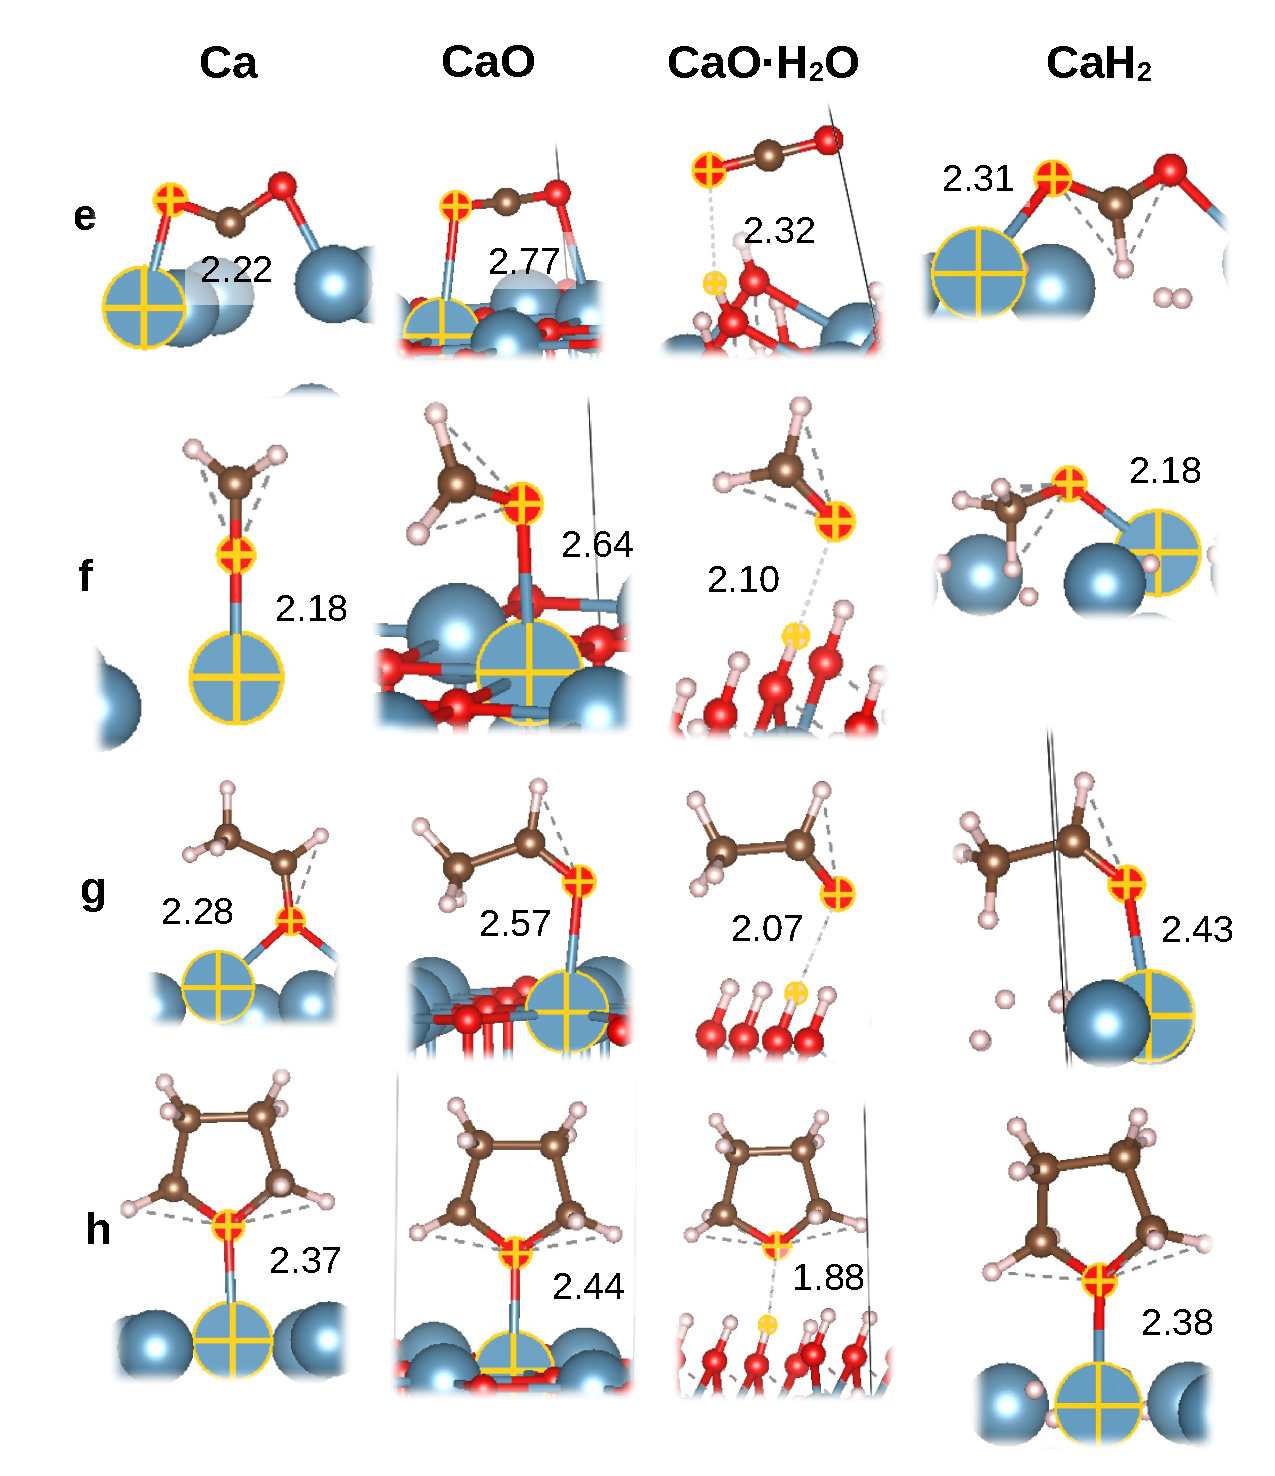
\includegraphics[width=.7\linewidth]{Figure7}
	\caption{Distances between adsorbate (hydrocabrons, \textbf{a}-\textbf{d}) and substrates, as measured by representative distances (in \si{\angstrom}) between one atom of each entity.}
	\label{fig:distsad}
\end{figure}

\begin{figure}[!h]
\centering
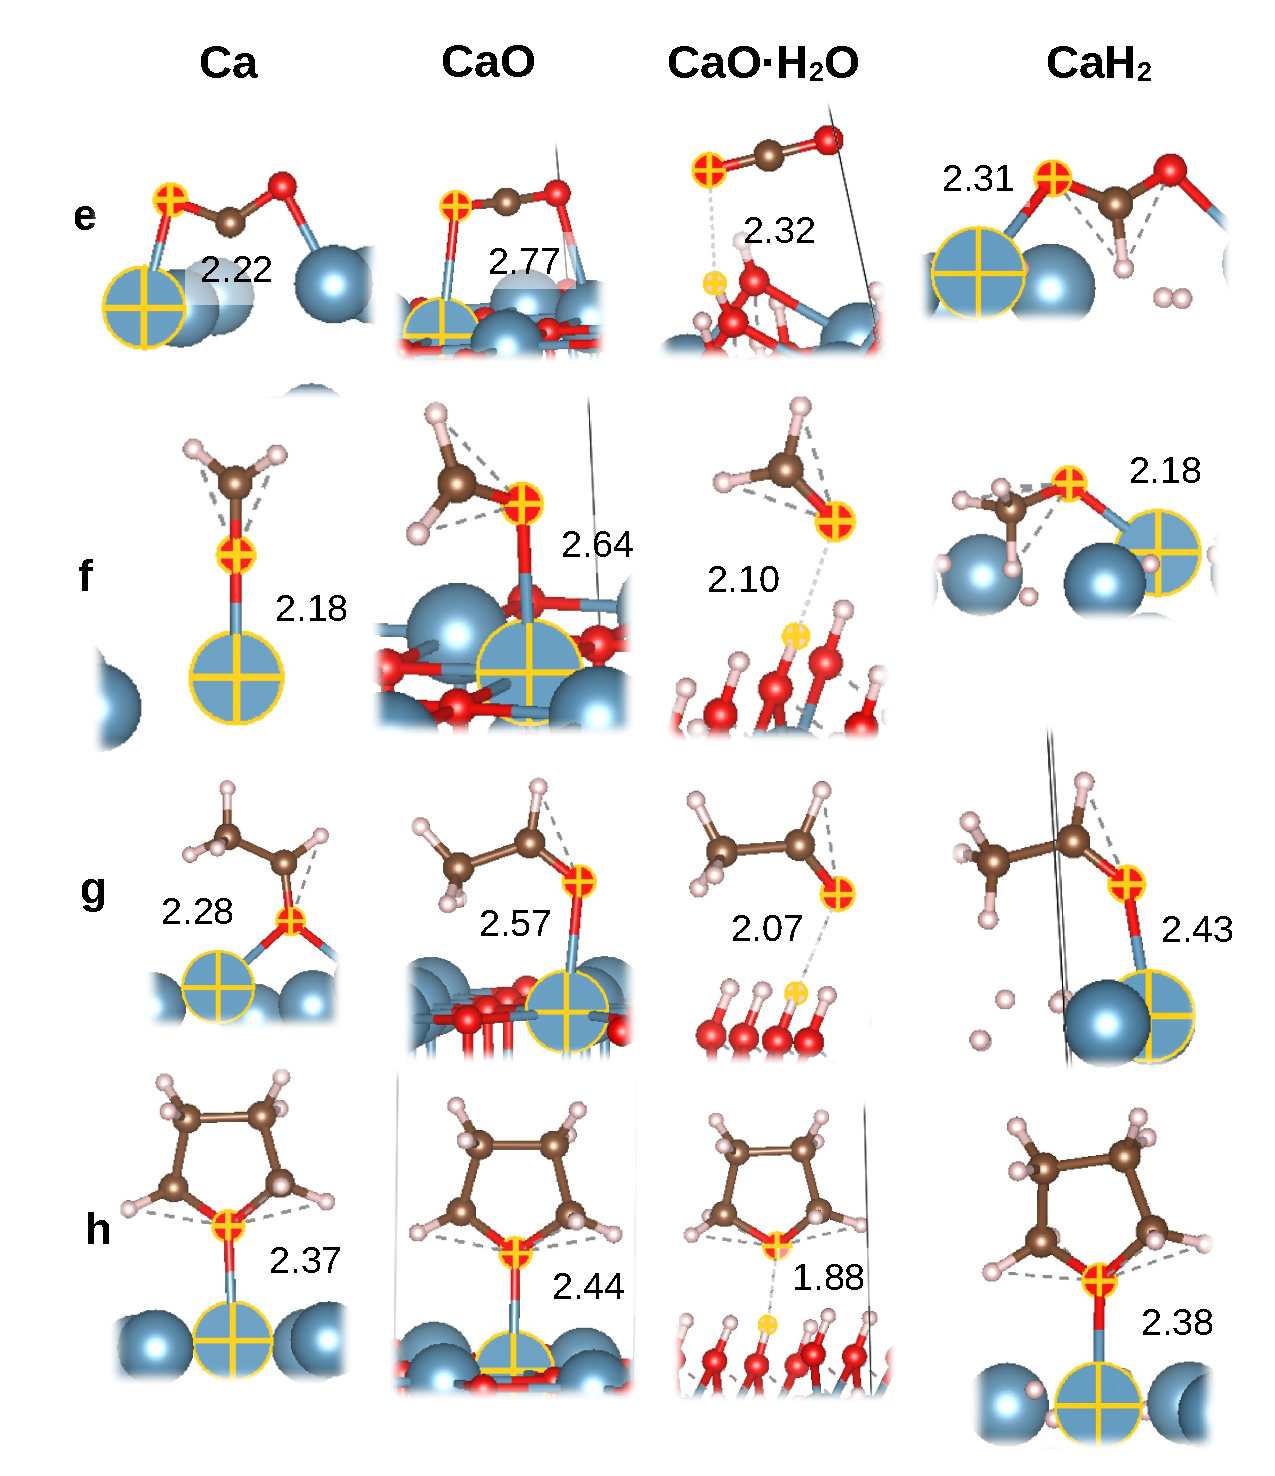
\includegraphics[width=.7\linewidth]{Figure8}
\caption{Distances between adsorbate (polar carbohydrates, \textbf{e}-\textbf{h}) and substrates, as measured by representative distances (in \si{\angstrom}) between one atom of each entity.}
\label{fig:distseh}
\end{figure}

\begin{figure}[!h]
\centering
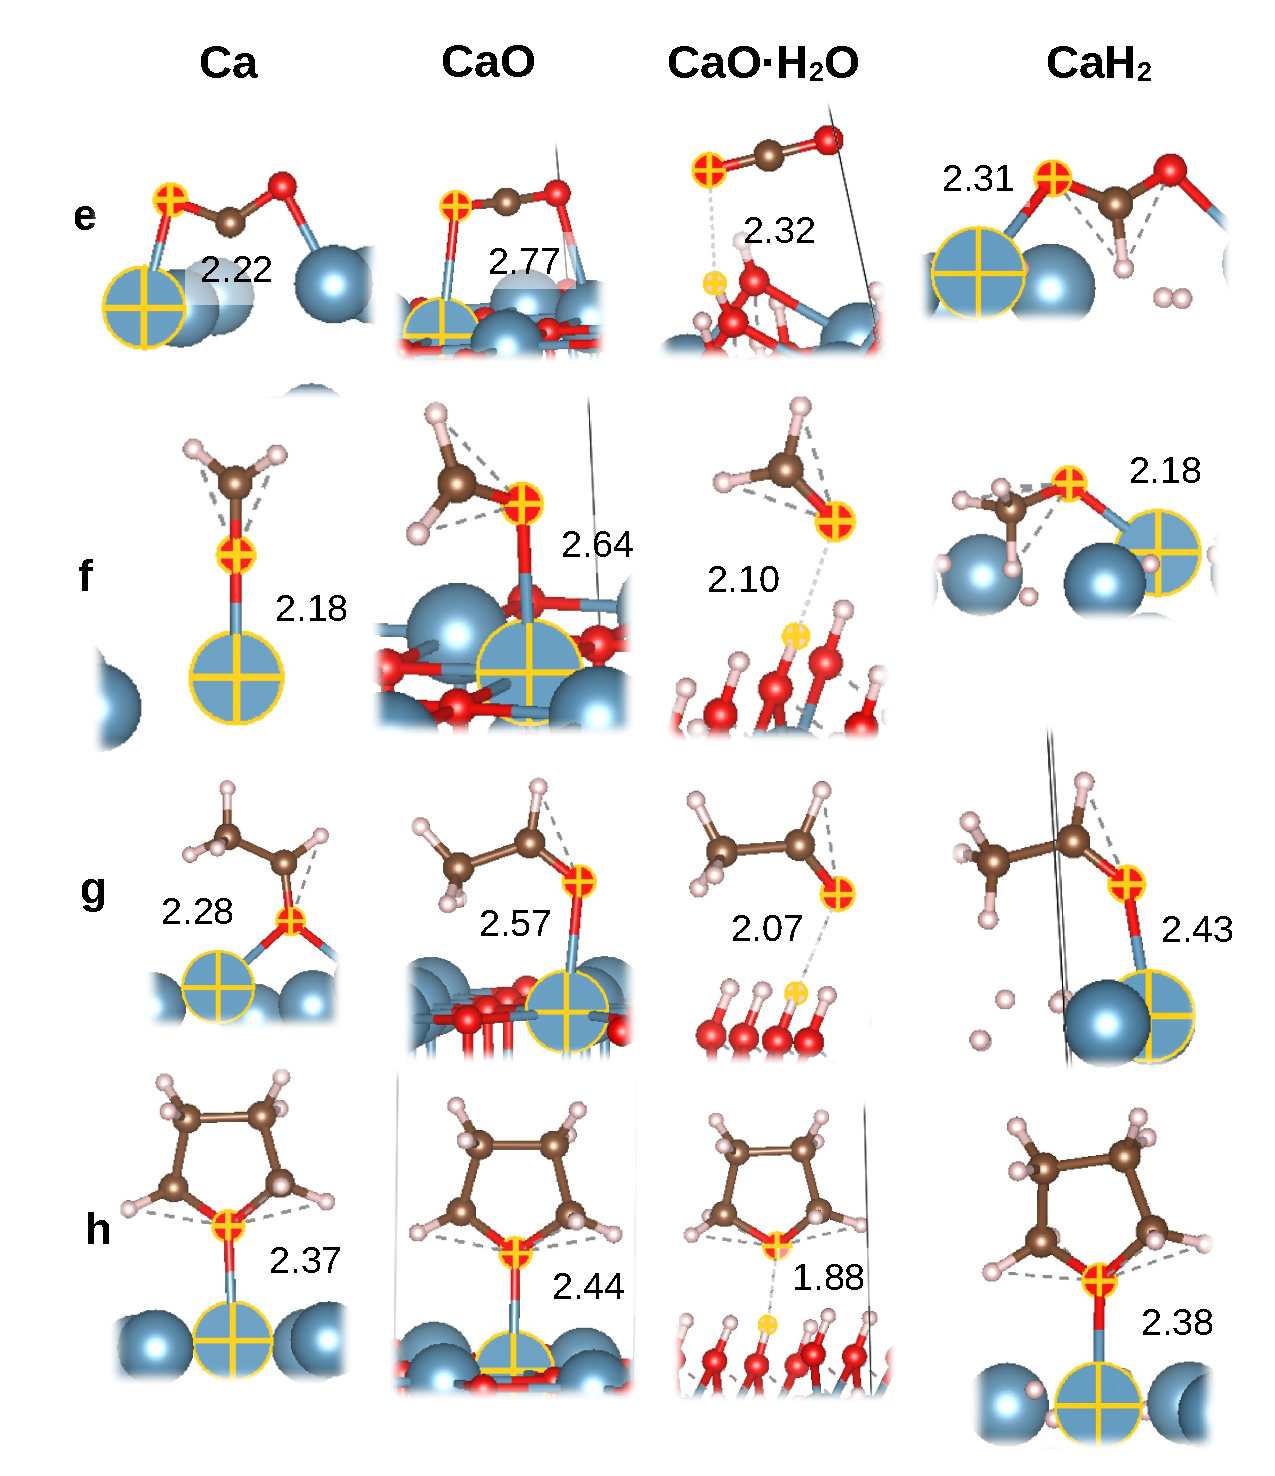
\includegraphics[width=.7\linewidth]{Figure9}
\caption{Distances between adsorbate (protic carbohydrates, \textbf{i}-\textbf{j}) and substrates, as measured by representative distances (in \si{\angstrom}) between one atom of each entity.}
\label{fig:distsij}
\end{figure}

\begin{table}[!h]
	\centering
	\begin{tabular}{>{\bfseries}lcccc}
		\toprule
		& Ca & \ce{CaO} & \ce{CaO.H2O} & \ce{CaH2} \\
		\midrule
		& \multicolumn{4}{c}{Hydrocarbons} \\
		a & -101.5 & -60.2 & -40.8 & -67.0 \\
		b & -111.2 & -78.9 & -56.2 & -76.0 \\
		c & -137.6 & -69.7 & -38.4 & -91.4 \\
		d & -140.7 & -89.8 & -52.5 & -96.9 \\
		\midrule
		& \multicolumn{4}{c}{Polar carbohydrates} \\
		e & -430.6 & -62.6 & -30.9 & -198.1 \\
		f & -239.4 & -70.9 & -34.4 & -302.1 \\
		g & -321.3 & -109.4 & -44.8 & -145.9 \\
		h & -215.3 & -121.6 & -55.6 & -152.6 \\
		\midrule
		& \multicolumn{4}{c}{Protic carbohydrates} \\
		i & -223.2 & -207.4 & -121.5 & -176.9 \\
		j & -475.4 & -532.5 & -223.8 & -437.6 \\
		\bottomrule
	\end{tabular}
	\caption{Interaction energy ($\Delta E_{int}$, in \si{\kilo\joule\per\mole}) between the adsorbate and the substrate.}
	\label{tab:int}
\end{table}

\clearpage
\subsection{Binding energies of adsorbate on slabs}

Since directly comparing molecules in the gas phase with those adsorbed on a slab is methodologically questionable (\textit{vide infra}), the binding energies before and after adsorption will be discussed. For the former, the geometries where the molecules are \SI{6}{\angstrom} from the slab surface are used. The XPS spectra of the adsorbates (computed using the results where these molecules are on top of bare Ca) are analyzed in Fig.~\ref{fig:adsorbare}. The C 1s spectra can be divided into three parts (in agreement with the trends reported in Fig.~\ref{fig:trends}): \begin{inparaenum}[i)]
	\item unsaturated carbons, with the lowest binding energies (\textit{e.g.}, \textbf{c} and \textbf{d}),
	\item aliphatic carbons (\textit{e.g.}, \textbf{a} and \textbf{b}), and
	\item carbons with neighboring oxygen atoms, with the highest binding energies (\textit{e.g.}, \textbf{g}).
\end{inparaenum}
Similarly, the O 1s spectra can be divided into two categories, depending on the hybridization of the oxygen. The lowest binding energies are associated with \ce{C=O} (\textit{e.g.}, \textbf{f} and \textbf{g}).

Two important observations should be noted: first, these binding energies are lower than those predicted in the gas phase.\footnote{Encore une fois, comparaison casse-gueule ;)} It is difficult at this time to determine whether this is due to the methodology (SJ vs. SJ\textsuperscript{n}, $E_F$ or not) or the presence of the Ca slab. One way to address this question would be to study the impact of the distance between the molecule and the slab. Second, the results for \textbf{e} (\ce{CO2}) do not follow the aforementioned trends (its O 1s binding energy is surprisingly large), indicating that further investigation definitely is required (could it be that since it is smaller, it feels less the slab?).

\begin{figure}[!h]
	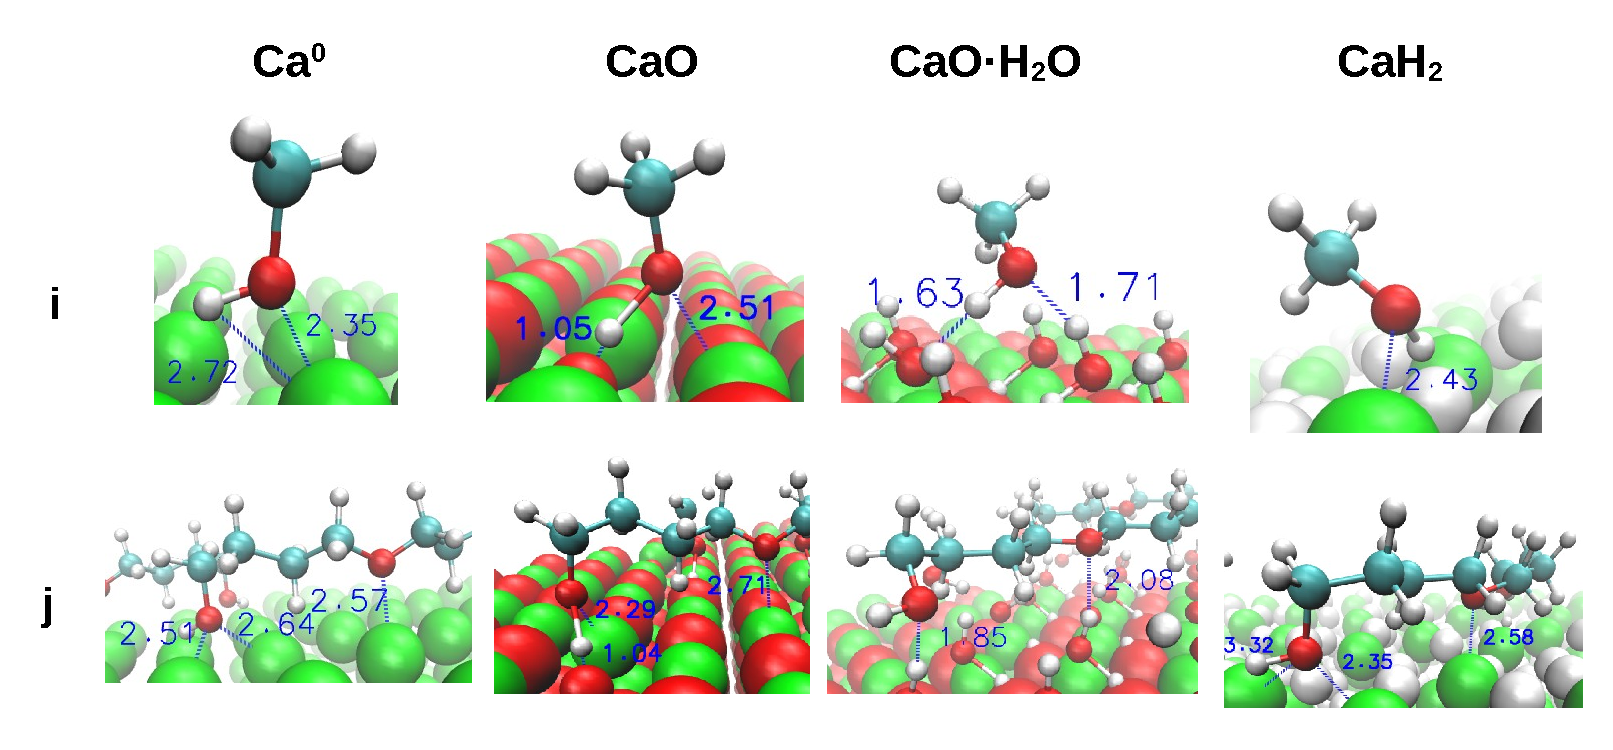
\includegraphics[width=\linewidth]{Figure10}
	\caption{XPS spectra (as computed with the SJ protocol) of the adsosorbates \textbf{a}-\textbf{j} before adsorption.}
	\label{fig:adsorbare}
\end{figure}

\clearpage

The impact of adsorption on binding energies is detailed in Figs.~\ref{fig:spectraXPSadsab}-\ref{fig:spectraXPSadsij}. For Ca 2s, adsorption-induced changes are minimal, with slightly more noticeable effects on the CaO slab, though not significant enough to be detectable experimentally. However, more substantial changes are observed for the other atoms studied: 
First, interaction with bare Ca results in a shift to lower binding energies in C 1s and a shift to higher binding energies in O 1s (when available), indicating electron transfer between the slab and the adsorbate. This suggests that interactions with hydrocarbons may involve more than just van der Waals forces. Then, hydrogen bond formation at the surface of \ce{CaO.H2O} causes a slight shift to higher O 1s \dbe{}, which increases with the strength of the bond (\textit{e.g.}, \textbf{f}-\textbf{h}).
Furthermore, proton transfers, seen in the interactions between \textbf{e} and \textbf{f} with \ce{CaH2} and between \textbf{i} and \textbf{j} with CaO, lead to significant changes in C 1s and O 1s binding energies, consistent with changes in hybridization. Finally, C 1s binding energies also change when unsaturated hydrocarbons (\textbf{c} and \textbf{d}) interact with \ce{CaH2}, suggesting a modification of the carbon's chemical environment, which may not be immediately apparent when inspecting the geometries.
These findings demonstrate that XPS binding energies are highly sensitive to changes in the chemical environment of the atoms.

\clearpage
\section{Conclusions}
XPS offers valuable insights into the chemical environment of atoms and the changes they undergo during adsorption. However, careful consideration must be given to the methodologies employed, as direct comparisons between results can be challenging due to potential inconsistencies across different systems.

To address these concerns, a thorough assessment of the methodology is necessary. Key considerations include, first, the impact of distance beetween slab and adsorbate The effect of the separation between the slab and the adsorbate on the \dbe{} should be thoroughly investigated. This examination is crucial to establish a clear connection to gas phase results and ensure accurate interpretations.
Then, the application of the SJ\textsuperscript{n} methodology. The SJ\textsuperscript{n} approach should be explored for adsorbates as well. The discussion around Fig.~\ref{fig:slabsthicknessSJn} suggests that SJ\textsuperscript{n} provides a better estimate of \dbe{} for CaO slabs. Confirmation of this finding could improve the reliability of \dbe{} predictions for various systems.

Once the methodology is validated, a deeper analysis of the experimental data provided by Prof. A. Vlad can be undertaken (thought we already have some insights). These data includes spectra for aging over different periods of time, which could provide insights into the kinetics of the degradation process. IR spectroscopy will enhance this analysis, when possible.

Furthermore, another objective is to investigate the behavior of \ce{BH4} and \ce{BF4} ions, aligning with the goals of the ECOBAT project. By integrating these investigations, a comprehensive understanding of the adsorption processes and chemical transformations in these systems can be achieved.


\clearpage
\bibliography{biblio}
	
\end{document}